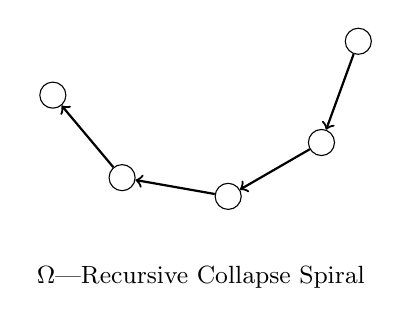
\begin{tikzpicture}[
    event/.style={circle, draw=black, fill=white, minimum size=4pt},
    arrow/.style={->, thick}
]

\foreach \i in {0,1,2,3,4}{
  \node[event] (e\i) at ({2*cos(\i*40)},{-2*sin(\i*40)}) {};
  \ifnum\i>0
     \draw[arrow] (e\the\numexpr\i-1\relax) -- (e\i);
  \fi
}

\node at (0,-3) {\small $\Omega$---Recursive Collapse Spiral};

\end{tikzpicture}